\setAuthor{Uku Andreas Reigo}
\setRound{lahtine}
\setYear{2023}
\setNumber{G 10}
\setDifficulty{10}
\setTopic{TODO}

\prob{Kõver trajektoor}
\begin{wrapfigure}{r}{0pt}
    \vspace{-50pt}
    \raisebox{-50pt}[0.5\dimexpr\height][-10000pt]{\magnetvali{}}    
    \vspace{-500pt}
\end{wrapfigure}



Elektron massiga $m$ ja laenguga $q$ alustab liikumist punkis $(0,h)$ kiirusega $v$ (vt joonis), kusjuures kiirusvektori ja y-telje sihi vaheline nurk on $\alpha$ nii, et $0<\alpha<\frac{\pi}{4}$. Milline peab olema magnetväljade tugevuste suhe $\frac{B_1}{B_2}$, et elektroni edasine trajektoor oleks kinnine ning ennast mitte lõikav?


\hint

\solu
Et trajektoor on kinnine ja ülesanne on mitmes mõttes sümmeetriline (näiteks laengu ja algse suuna vahetamise korral peaks töötama, lisaks ka olukorra peegeldamisel üle sirge y=x), siis on näha, et nurk kiirusvektori ja x-telje vahel, kui elektron lahkub 1. veerandist, on samuti $\alpha$.

Edaspidi annan kõik nurgad positiivse x-telje suhtes vastupäeva mõõdetuna. 

%TODO korruta -1-ga, et tuleks positiivne osa ringist.
Algne nurk on $\theta_1 = \frac{\pi}{2} - \alpha$. 1. sektorist väljudes on nurk $\theta_2 = \alpha - \pi$, ehk $\Delta\theta = 2\alpha - \frac{3\pi}{2}$, seega sealne trajektoori osa moodustab $\frac{2\alpha-\frac{3\pi}{2}}{2\pi} = \frac{\alpha}{\pi} - \frac{3}{4}$ ringist. Järeldub ka, et kesknurk sisenemis- ja väljumispunkti vahel 1. sektoris on $\gamma = \frac{\pi}{2} + 2\alpha$

Samuti sümmeetriast teame, et trajektoor lõikab x-telge punktis $(h,0)$. Seega on sisenemis- ja väljumispunkti ühendava kõõlu pikkus $L = \sqrt{2}h$ ning ringi raadius $R_2 = \frac{L}{2\sin{\frac{\gamma}{2}}} = \frac{\sqrt{2}h}{2\sin{(\frac{\pi}{4}+\alpha)}}$



\begin{figure}[h]
    \centering
    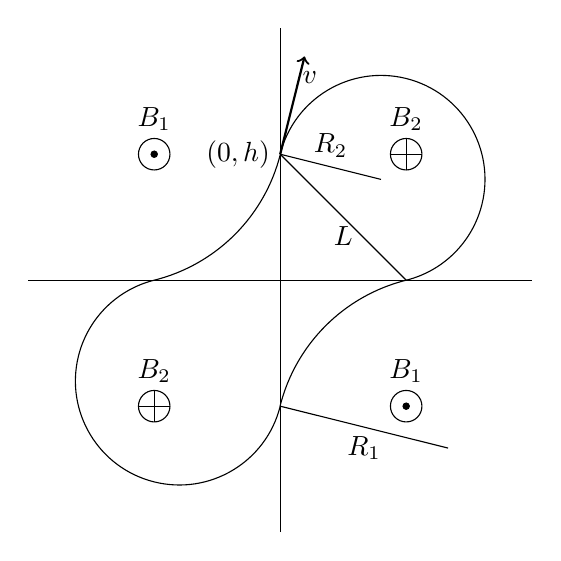
\begin{tikzpicture}[scale = 0.8]
        \draw (-4,0) -- (4,0);
        \draw (0,-4) -- (0,4);

        \draw[thick,->] (0,2) node [anchor = east] {$(0,h)$}
                            -- ++(76:1.6)
                            node [midway, yshift=10, anchor = west] {$\Vec{v}$};

        \draw (-2,2) circle (0.25) node[above, anchor = south, yshift = 5] {$B_1$};
        \filldraw (-2,2) circle (0.05);
        
        \draw (2,-2) circle (0.25) node[above, anchor = south, yshift = 5] {$B_1$};

        \filldraw (2,-2) circle (0.05);

        \draw (2,2) circle (0.25) node[above, anchor = south, yshift = 5] {$B_2$};
        \draw (2.25,2) -- (1.75,2);
        \draw (2,1.75) -- (2,2.25);

        \draw (-2,-2) circle (0.25) node[above, anchor = south, yshift = 5] {$B_2$};

        \draw (-2.25,-2) -- (-1.75,-2);
        \draw (-2,-1.75) -- (-2,-2.25);

        

        \draw (0,2) arc (166:-76:1.65);
        \draw (2,0) arc (104:166:2.75);
        \draw (0,-2) arc (-14:-256:1.65);
        \draw (-2,0) arc (-76:-14:2.75);

        \draw (0,2) -- (1.6,1.6) node[midway, above]{$R_2$};
        \draw (2.665,-2.665) -- (0,-2) node[midway, below]{$R_1$};
        \draw (0,2) -- (2,0) node [midway, below]{$L$};
    \end{tikzpicture}
    \caption*{Näidislahend $a = 14^\circ$ korral. $R_2 \approx 0.83 h$ ja $R_1 \approx 1.38 h$}
\end{figure}

2. sektoris viib sarnane arutelu arusaamani, et nurk muutub väärtuselt $\theta_2 = \alpha - \pi$ väärtuseni $\theta_3 = \frac{-\pi}{2} - \alpha$, läbides nurga $\Delta\theta = \frac{\pi}{2} - 2\alpha$. Seega kesknurk sisenemis- ja väljumispunkti vahel on $\gamma = \frac{\pi}{2} - 2\alpha$. Neid punkte ühendava kõõlu pikkus on jälle $L = \sqrt{2}h$ ning raadius $R_1 = \frac{L}{2\sin{\frac{\gamma}{2}}} = \frac{\sqrt{2}h}{2\sin{(\frac{\pi}{4}-\alpha)}}$

Et magnetväljas tiirleva elektroni tiirlemisraadius $R = \frac{mv}{qB}$, siis $\frac{R_1}{R_2} = \frac{B_2}{B_1} = \frac{\sin(\frac{\pi}{4}+\alpha)}{\sin{(\frac{\pi}{4}-\alpha)}}$
\probend